\label{chap.5}
\section{Motivation and Objective}
Self-supervised learning (SSL) learns representations from network telemetry without needing a label for every observation. The idea in this project was that such representations could feed the later stages, a classifier or the forecaster, and that they would help most when labelled data is scarce. This chapter tests that idea honestly: it describes the encoder, the data problems that first made the results look worse than they were, and a label-efficiency study that asks the question SSL is meant to answer, namely whether pretraining helps when only a few flows are labelled.

\section{Pretext Tasks}
\subsection{First implementation: masked reconstruction}
The first encoder was trained on the 5G-NIDD dataset. Eleven context features (protocol, TCP state, TTL and hop attributes, among others) were treated as categorical variables with an 8-dimensional embedding each. Fourteen volume and rate features (packet and byte counts, mean packet sizes, load and rate) were masked at a ratio of 0.30 and reconstructed from the visible context. The encoder had two linear layers of 128 and 64 units and produced a 64-dimensional embedding; a decoder with a hidden layer of 128 units reconstructed the masked values. The loss is the mean squared error over the masked positions only,
\begin{equation}
\mathcal{L}_{\mathrm{mask}} = \frac{1}{|\mathcal{M}|}\sum_{j\in\mathcal{M}}(\hat{x}_j-x_j)^2 ,
\label{eq:mask_loss}
\end{equation}
where $\mathcal{M}$ is the set of masked positions, $x_j$ the original value and $\hat{x}_j$ the reconstruction. Training used Adam with a learning rate of $10^{-3}$, a batch size of 512 and 10 epochs, on all 1.2 million flows.

\subsection{Re-evaluation: two pretext tasks on cleaned data}
For the final study the pretraining was redone with two standard tabular pretext tasks, using one encoder shape (83 inputs, two hidden layers of 256 units, a 64-dimensional output) so that the comparison between them is fair.
\begin{itemize}
\item \textbf{Masked-feature modelling.} Thirty per cent of the entries of every flow are replaced by the values of the same feature in other flows, and the encoder must reconstruct the original values and also detect which entries were replaced \cite{yoon2020vime}.
\item \textbf{Contrastive learning (SCARF).} Each flow is paired with a copy in which 60\% of the features are replaced by values from random other flows, and a contrastive loss over the batch (temperature 0.5, batch size 512) pulls the two views together \cite{bahri2022scarf}.
\end{itemize}
Both were trained without any label on the 80\% pool of flows kept for training (326{,}924 flows).

\section{Cleaning the Data}
The first evaluation reported a macro-F1 of 0.708. Two data problems explain why that number was so low, and fixing them changed the baseline far more than any SSL variant.
\begin{itemize}
\item \textbf{Duplicate flows.} Of the 1{,}215{,}890 flows in 5G-NIDD, 807{,}235 (66\%) are exact copies, so a random split puts identical flows in the training and the test set. After removing them, 408{,}655 unique flows remain, in nine classes (benign and eight attack types).
\item \textbf{Identifier columns.} The row index, the sequence number and the offset identify a flow's position in the capture and leak its label, so they were removed. The remaining numeric features are heavy-tailed counts, so they were log-scaled, and the categorical features were one-hot encoded, giving 83 inputs.
\end{itemize}
A stratified 80/20 split gives a pretraining pool of 326{,}924 flows and a test set of 81{,}731 flows. A further problem was found earlier: the source file is stored in blocks of identical labels, so a split by position put 99.88\% of one class in the test set and gave an accuracy of about 1\%. The stratified split removed that problem too.

\section{Label-Efficiency Study}
Pretraining is expected to help when labels are scarce, so classifiers were trained with 50, 200, 1{,}000, 5{,}000 and 20{,}000 labelled flows and with all labels. Each budget up to 5{,}000 was repeated with five random label draws (two above that). The classifiers were: logistic regression, a small multilayer perceptron and LightGBM 	te{ke2017lightgbm} on the raw features; logistic regression on the frozen embedding; the pretrained encoder fine-tuned with a classification head; and logistic regression on the raw features concatenated with the embedding. The metric is the macro-averaged F1 over the nine classes.

\begin{table}[htbp]
\centering
\caption{Macro-F1 on 81{,}731 unseen 5G-NIDD flows, by number of labelled flows (mean of five label draws up to 5{,}000 labels, two above)}
\label{tab:ssl_label_efficiency}
\footnotesize
\begin{tabular}{|>{\centering\arraybackslash}p{\dimexpr 0.108\textwidth-2\tabcolsep\relax}|>{\centering\arraybackslash}p{\dimexpr 0.108\textwidth-2\tabcolsep\relax}|>{\centering\arraybackslash}p{\dimexpr 0.108\textwidth-2\tabcolsep\relax}|>{\centering\arraybackslash}p{\dimexpr 0.108\textwidth-2\tabcolsep\relax}|>{\centering\arraybackslash}p{\dimexpr 0.108\textwidth-2\tabcolsep\relax}|>{\centering\arraybackslash}p{\dimexpr 0.108\textwidth-2\tabcolsep\relax}|>{\centering\arraybackslash}p{\dimexpr 0.108\textwidth-2\tabcolsep\relax}|>{\centering\arraybackslash}p{\dimexpr 0.108\textwidth-2\tabcolsep\relax}|>{\centering\arraybackslash}p{\dimexpr 0.108\textwidth-2\tabcolsep\relax}|}
\hline
\textbf{Labels} & \textbf{LGBM raw} & \textbf{MLP raw} & \textbf{Logit raw} & \textbf{Masked emb.} & \textbf{Masked fine-tuned} & \textbf{SCARF emb.} & \textbf{SCARF fine-tuned} & \textbf{Raw + SCARF} \\ \hline
50 & 0.643 & 0.694 & 0.704 & 0.627 & 0.684 & 0.594 & 0.688 & 0.690 \\ \hline
200 & 0.852 & 0.858 & 0.853 & 0.763 & 0.834 & 0.713 & 0.850 & 0.848 \\ \hline
1{,}000 & 0.905 & 0.895 & 0.874 & 0.859 & 0.881 & 0.842 & 0.894 & 0.888 \\ \hline
5{,}000 & 0.919 & 0.911 & 0.909 & 0.901 & 0.898 & 0.880 & 0.901 & 0.915 \\ \hline
20{,}000 & 0.932 & 0.924 & 0.923 & 0.913 & 0.923 & 0.907 & 0.925 & 0.924 \\ \hline
all & 0.936 & 0.925 & 0.926 & 0.912 & 0.927 & 0.910 & 0.929 & 0.926 \\ \hline
\end{tabular}
\end{table}

\begin{figure}[htbp]
\centering
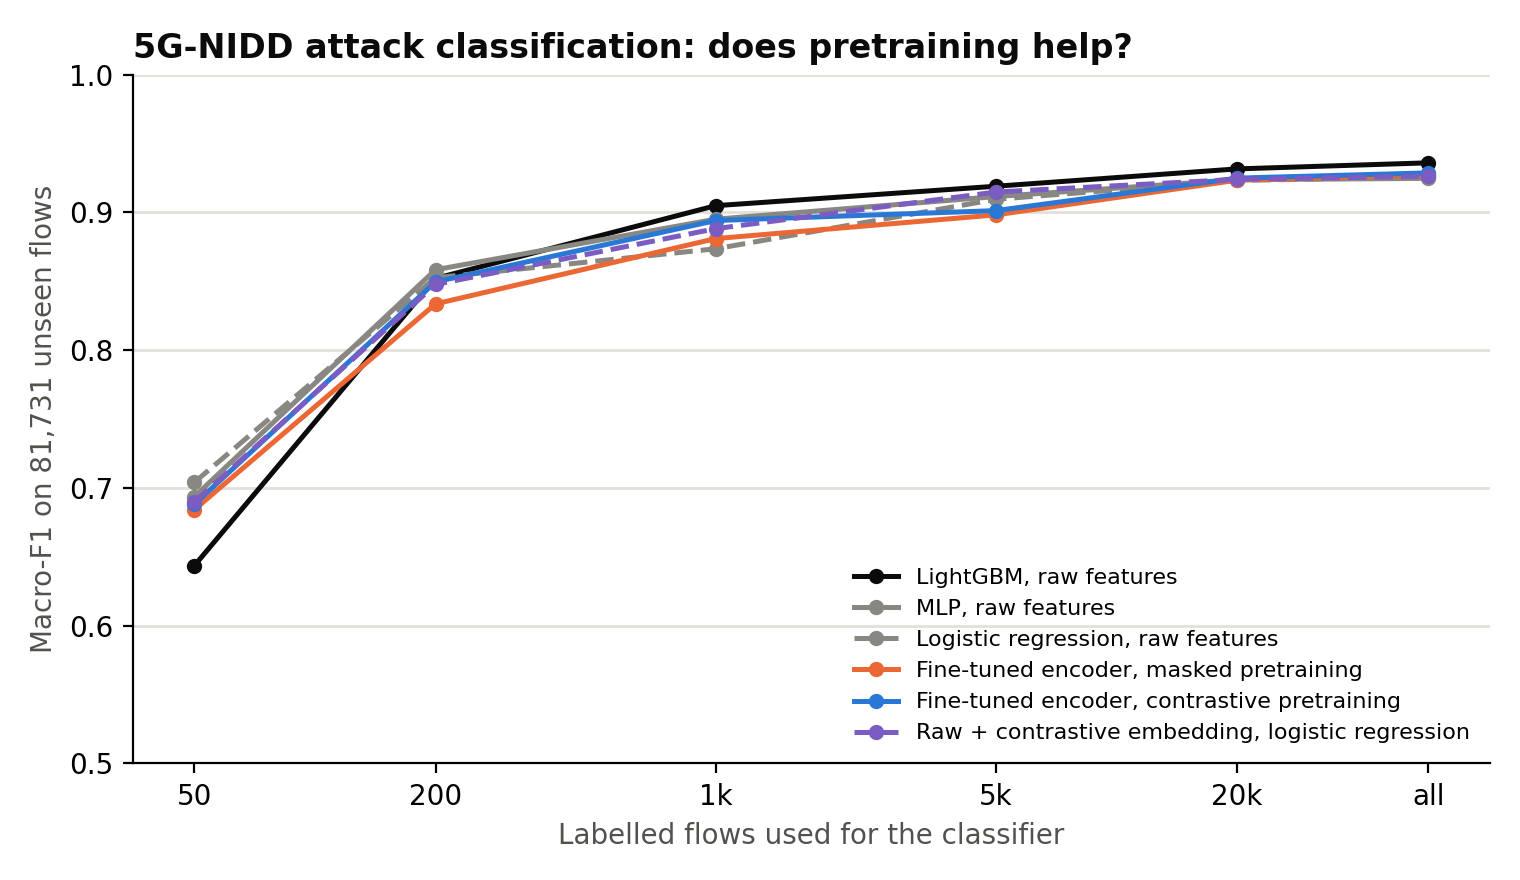
\includegraphics[width=0.9\textwidth,keepaspectratio]{unified_ssl_label_efficiency.png}
\caption{Macro-F1 against the number of labelled flows for raw features and pretrained encoders}
\label{fig:ssl_label_efficiency}
\end{figure}

Three observations follow from Table~\ref{tab:ssl_label_efficiency} and Figure~\ref{fig:ssl_label_efficiency}.
\begin{enumerate}
\item The raw features are already strong. Logistic regression reaches 0.926 and LightGBM 0.936 with all labels, against 0.708 in the first evaluation, so most of the earlier gap came from duplicates and leaked identifiers rather than from the classifier.
\item Pretraining does not beat the best raw-feature model at any budget. With 50 and 200 labels a raw-feature multilayer perceptron or logistic regression is ahead of the fine-tuned encoder (for example 0.694 and 0.704 against 0.688 at 50 labels), and a linear classifier on the frozen embedding alone is clearly worse. With all labels the fine-tuned contrastive encoder ties the same network trained from scratch (0.929 against 0.925) and stays below LightGBM.
\item Adding the embedding to the raw features helps a linear model only a little, by at most 0.014 at 1{,}000 to 5{,}000 labels, and not at all with 20{,}000 or more.
\end{enumerate}
LightGBM is the weakest method at 50 labels because boosted trees need more data, which is why the comparison above is made against the neural and linear raw-feature models as well.

\section{SSL on the Milan Forecast}
\label{sec:milan_ssl}
In the first forecasting experiment (Chapter~\ref{chap.6}) a TGNN fed with 64-dimensional embeddings of Milan traffic features scored the same validation error as one fed with the raw features (0.000616 against 0.000612). That was a single day and a single seed, so it was repeated on the city forecaster. The embedding here is 16-dimensional and describes one cell's input window (the last six intervals of demand, the same time on the previous day, time of day and a weekend flag). An encoder is pretrained without labels by hiding 30\% of the entries of a window and reconstructing them, on windows from the training days only, then frozen and its output is given to the forecaster's output layer. Table~\ref{tab:ssl_milan} gives the outcome. Both variants use the same data, split, scaling and number of training steps; the only difference is the embedding. The pretrained embedding does not help: with it the eMBB improvement is about one percentage point lower (15\% against 16\%), and URLLC and mMTC are within half a point of the raw forecaster. Each variant was trained twice with different seeds, and the run-to-run difference is of the same size as the gap, so we conclude that the embedding adds nothing measurable.

\begin{table}[htbp]
\centering
\caption{City forecaster with and without a pretrained window embedding, improvement over persistence on the held-out week (eMBB / URLLC / mMTC)}
\label{tab:ssl_milan}
\footnotesize
\begin{tabular}{|>{\centering\arraybackslash}p{\dimexpr 0.194\textwidth-2\tabcolsep\relax}|>{\centering\arraybackslash}p{\dimexpr 0.194\textwidth-2\tabcolsep\relax}|>{\centering\arraybackslash}p{\dimexpr 0.194\textwidth-2\tabcolsep\relax}|>{\centering\arraybackslash}p{\dimexpr 0.194\textwidth-2\tabcolsep\relax}|>{\centering\arraybackslash}p{\dimexpr 0.194\textwidth-2\tabcolsep\relax}|}
\hline
\textbf{Forecaster input} & \textbf{Runs} & \textbf{eMBB} & \textbf{URLLC} & \textbf{mMTC} \\ \hline
Raw inputs (the city forecaster as it is) & 2 & +16\% & +32\% & +31\% \\ \hline
Raw inputs + frozen 16-dimensional SSL embedding & 2 & +15\% & +32\% & +31\% \\ \hline
\end{tabular}
\end{table}

\section{Interpretation}
\label{sec:ssl_interpretation}
The finding is the same on both tasks: the raw features already hold what the downstream models need, and masked or contrastive pretraining adds very little. A likely reason is that these are low-dimensional, hand-made features and not raw packets or long sequences. Pretraining is known to pay off on high-dimensional raw inputs, where no one has engineered features. Other work on tabular data reports the same thing, namely that the advantage of pretraining often disappears against well-tuned baselines \cite{rubachev2022revisiting}. We therefore report SSL as a negative result of this project. What this chapter contributes is the cleaned evaluation: de-duplicated data, no leaked columns, a design that varies the number of labels, and strong raw-feature baselines. The SSL stage stays in the pipeline of Chapter~\ref{chap.4} because the literature recommends it, but we do not claim that it improves the forecasts or the allocation.
